\documentclass{article}

\usepackage{tikz}
\usepackage{xcolor}
\usepackage{pgfplots}
\usepackage{ifthen}
\usepackage{multicol}
\usepackage{xcolor}
\usepackage{array}
\usepackage{colortbl}
\usepackage{lipsum}
\usepackage{hulipsum}
\usepackage{blindtext}
\usepackage{amsmath}
\usepackage{ifthen}
\usepackage{intcalc}

\usetikzlibrary{patterns}
\usetikzlibrary{shapes.geometric, arrows}
\usetikzlibrary{positioning}

\begin{document}

\newenvironment{vonalzott}
{\vspace{1ex}\hrule\vspace{1ex}}
{\vspace{1ex}\hrule\vspace{1ex}}

\newenvironment{kulcsgondolatok}[1][Kulcsgondolatok]{
    \par\noindent\hrulefill\par
    \begin{center}
    \begin{minipage}{0.8\textwidth}
    \centering
    \textbf{\large #1}\par
    \vspace{0.5em}
    \hrule
    \vspace{0.5em}
}{
    \end{minipage}
    \end{center}
    \hrule
}

elso
\begin{vonalzott}
kozep
\end{vonalzott}
hatso

\begin{kulcsgondolatok}
\hulipsum[1-2]
\end{kulcsgondolatok}
\newpage

\begin{tabular}{ccc}
\arrayrulecolor{white} \hline
\rowcolor[HTML]{FFFFFF} a & b & c \\
\arrayrulecolor{white} \hline
\rowcolor[HTML]{858585} \textcolor{white}{a} & \textcolor{white}{b} & \textcolor{white}{c} \\
\arrayrulecolor{white} \hline
\rowcolor[HTML]{FFFFFF} a & b & c \\
\arrayrulecolor{white} \hline
\rowcolor[HTML]{858585} \textcolor{white}{a} & \textcolor{white}{b} & \textcolor{white}{c} \\
\arrayrulecolor{white} \hline
\rowcolor[HTML]{FFFFFF} a & b & c \\
\arrayrulecolor{white} \hline
\end{tabular}

\begin{tabular}{ccc}
\arrayrulecolor{white} \hline
\rowcolor[HTML]{FFFFFF} \textcolor{blue}{a} & \textcolor{blue}{b} & \textcolor{blue}{c} \\
\arrayrulecolor{white} \hline
\rowcolor[HTML]{FFFFFF} \textcolor{red}{a} & \textcolor{red}{b} & \textcolor{red}{c} \\
\arrayrulecolor{white} \hline
\rowcolor[HTML]{FFFFFF} \textcolor{blue}{a} & \textcolor{blue}{b} & \textcolor{blue}{c} \\
\arrayrulecolor{white} \hline
\rowcolor[HTML]{FFFFFF} \textcolor{red}{a} & \textcolor{red}{b} & \textcolor{red}{c} \\
\arrayrulecolor{white} \hline
\rowcolor[HTML]{FFFFFF} \textcolor{blue}{a} & \textcolor{blue}{b} & \textcolor{blue}{c} \\
\arrayrulecolor{white} \hline
\end{tabular}

\begin{enumerate}
    \foreach \x in {3,6,...,48} {
        \item \x
    }
\end{enumerate}

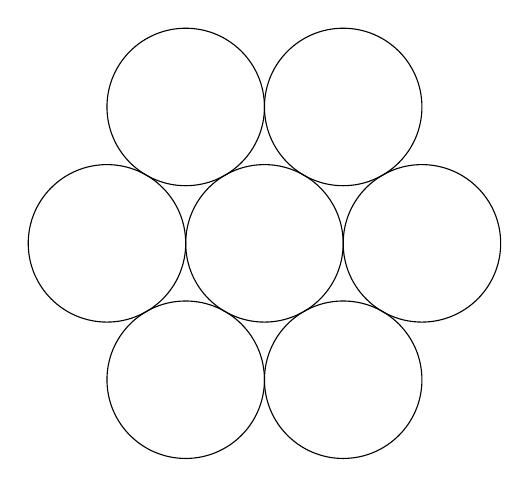
\begin{tikzpicture}
    \foreach \x/\y in {-2/0, 0/0, 2/0, -1/1.732, 1/1.732, -1/-1.732, 1/-1.732} {
        \draw (\x,\y) circle (1);
    }
\end{tikzpicture}

\begin{multicols}{4}
\newcounter{y}
\setcounter{y}{1}
\whiledo{\value{y}<61}{
    %\ifthenelse{\isodd{\value{y}}}
    \ifthenelse{\intcalcMod{\value{y}}{3}=0}
    		{\ifthenelse{\intcalcMod{\value{y}}{5}=0}
    				{\arabic{y}. cikk cakk\par}
    				{\arabic{y}. cikk\par}
    				}
        {\ifthenelse{\intcalcMod{\value{y}}{5}=0}
    				{\arabic{y}. cakk\par}
    				{\arabic{y}. \par}
    				}
    \stepcounter{y}
}
\end{multicols}

\end{document}